\documentclass[a4paper, 12pt]{article}

\usepackage[T1]{fontenc}

\usepackage{lipsum}
\usepackage{pifont}
\usepackage{amssymb}
\usepackage{amsmath}
\usepackage[utf8]{inputenc}
\usepackage[italian]{babel}
\usepackage{graphicx}
\graphicspath{ {./images/} }
\usepackage{spverbatim}
\usepackage{float}
\usepackage{url}
\usepackage{xstring}

\usepackage{hyperref}

\usepackage{xcolor}
\definecolor{linkcolor}{RGB}{1,1,87}
\hypersetup{
    colorlinks,
    citecolor=black,
    filecolor=black,
    linkcolor=linkcolor,
    urlcolor=blue
}
\usepackage{fancyvrb,newverbs,xcolor}
\definecolor{cverbbg}{gray}{0.93}

\newcommand{\makesub}[1]{%
  \saveexpandmode\noexpandarg
  \StrSubstitute{#1}{\_}{_}[\temp]%
  \restoreexpandmode%
}

\newcommand{\target}[1]{%
  \makesub{#1}%
  \hypertarget{\temp}{}%
}

\newcommand{\attach}[1]{%
  \makesub{#1}%
  \hyperlink{\temp}{\emph{#1}}%
}
\newcommand{\attachedCode}[1]{%
  \makesub{#1}%
  \hyperlink{\temp}{\code{#1}}%
}

\newcommand{\code}[1]{\colorbox{cverbbg}{\texttt{\StrSubstitute{#1}{_}{\_}}}}

\newcommand*\xor{\oplus}
\newcommand{\nota}[1]{\textbf{Nota}: #1}
\newcommand{\memo}[1]{\textbf{Memo}: #1}
\newcommand{\esempio}[1]{\textbf{Esempio}: #1}
\newcommand{\tbs}{\textbackslash}
\newcommand{\ghidra}{\emph{Ghidra}}
\newcommand{\ollydb}{\emph{OllyDB}}
\newcommand{\Null}{\code{NULL}}
\newcommand{\dll}{\emph{DLL}}
\newcommand{\api}{\emph{API}}
\newcommand{\key}[1]{\texttt{#1}}


\newenvironment{myverb}
 {\SaveVerbatim{cverb}}
 {\endSaveVerbatim
  \flushleft\fboxrule=0pt\fboxsep=.5em
  \colorbox{cverbbg}{%
    \makebox[\dimexpr\linewidth-2\fboxsep][l]{\BUseVerbatim{cverb}}%
  }
  \endflushleft
}

\setcounter{tocdepth}{4}
\setcounter{secnumdepth}{4}

\begin{document}\sloppy
  
\title{
  \textbf{
    \emph{Relazione homework 3}
  }
}  
\author{Luca Mastrobattista\\ Matricola: 0292461}
\date{}
\maketitle

\tableofcontents
\newpage
\section{Traccia dell'homework}
\subsection{Testo}
Analizzare con Ghidra e OllyDbg il programma eseguibile
hw3.exe contenuto nell'archivio hw3.zip.
Determinare il codice di sblocco che rende funzionale il
programma e riassumere in un documento tutte le informazioni
acquisite, la metodologia adottata ed i passi logici deduttivi
utilizzati nel lavoro di analisi.
\subsection{Scadenza}
Due settimane dalla data di assegnazione del lavoro: 13/12/2021.
\subsection{Consegna}
Documento in formato PDF inviato come allegato ad
un messaggio di posta elettronica all'indirizzo del docente
("$<$cognome$>$@uniroma2.it"), con subject:
"[AMW21] HW3: $<$matricola studente$>$"

\newpage
\section{Ambiente di lavoro}
Il file eseguibile è stato caricato su Ghidra istallato su un sistema operativo Linux. \\
L'ambiente controllato di utilizzo è un sistema operativo Windows 10 virtualizzato con il software \emph{VirtualBox}, in cui sono istallati gli strumenti di monitoraggio.


\newpage
\section{Metodologia}

\subsection{Informazioni note a priori}
Dalla traccia dell'\emph{homework} si deduce che l'eseguibile risulta \textit{bloccato} in qualche modo, e solo con un particolare codice si riesce a farlo funzionare correttamente.

\subsection{Finalizzazione dell'obiettivo}
L'analisi dell'applicazione ha come obiettivo quello di individuare il codice di sblocco.

\subsection{Ottenimento del codice macchina}
Codice macchina fornito dal professore.

\subsection{Osservazione del funzionamento}
L'applicazione, una volta avviata, crea una finestra con un \textit{countdown} impostato a 30 minuti per default, ma questo tempo è modificabile. Premendo sul pulsante \textit{Go}, il conto alla rovescia inizia. È presente una casella di testo in cui inserire il codice da trovare. 
\begin{figure}[H]
\centering 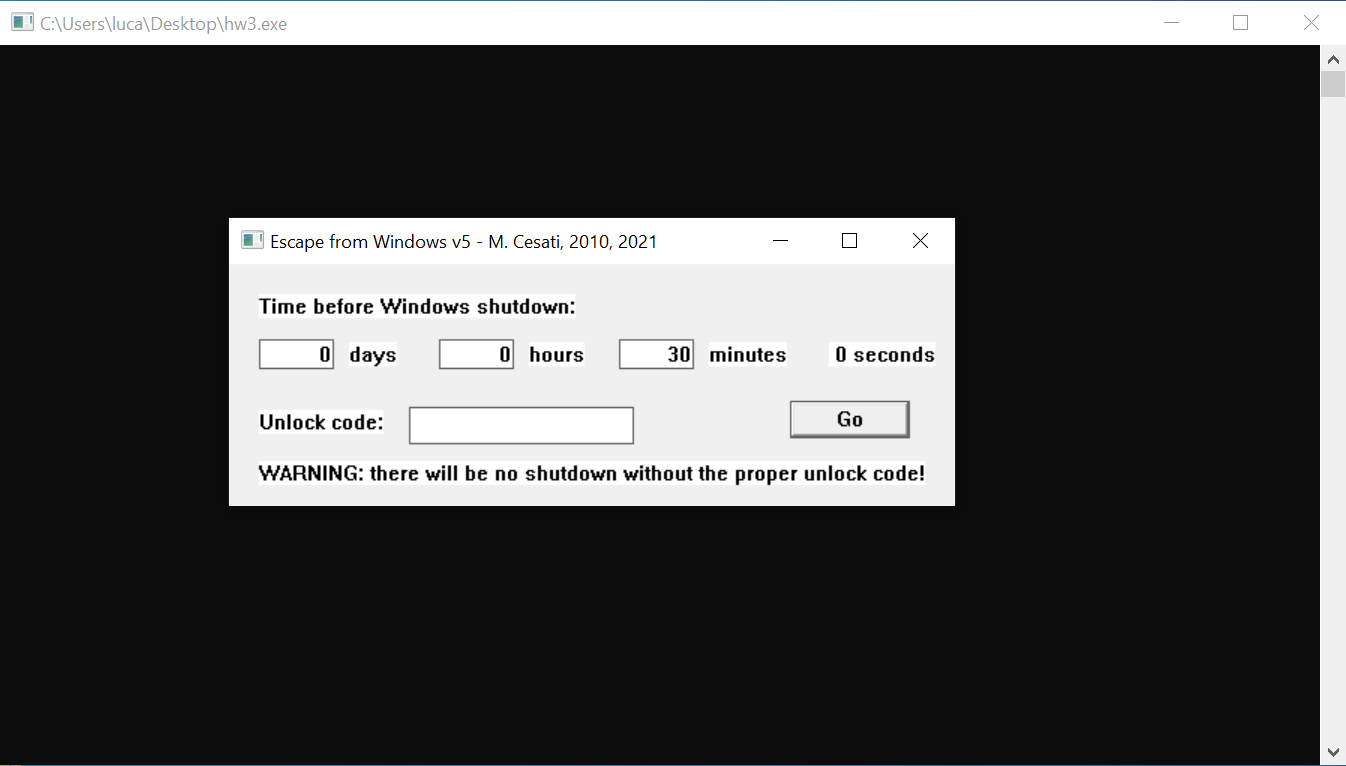
\includegraphics[scale=0.4]{program_launch}
\end{figure}
Al termine del \textit{countdown}, se il codice inserito non è corretto, compare una finestra di avviso di codice errato:
\begin{figure}[H]
\centering 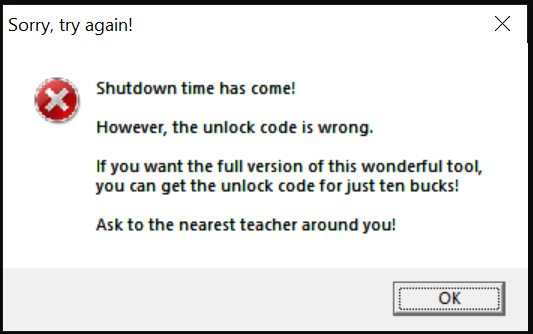
\includegraphics[scale=0.7]{error_message}
\end{figure}


\subsection{Disassemblaggio del codice macchina}
Lo strumento che si è utilizzato è il software \emph{Ghidra}.

\subsubsection{Riepilogo risultati dell'import}
\begin{figure}[H]
\centering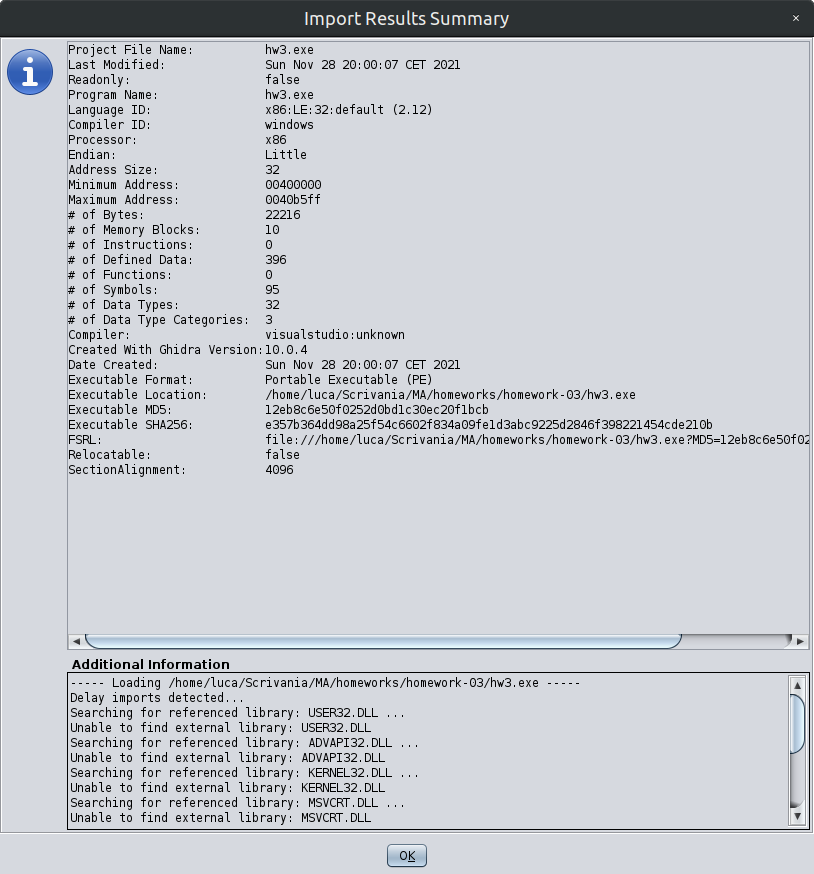
\includegraphics[width=\textwidth]{import}
\end{figure}


\subsubsection{Informazioni aggiuntive}
\begin{spverbatim}
----- Loading /home/luca/Scrivania/MA/homeworks/homework-03/hw3.exe -----
Delay imports detected...
Searching for referenced library: USER32.DLL ...
Unable to find external library: USER32.DLL
Searching for referenced library: ADVAPI32.DLL ...
Unable to find external library: ADVAPI32.DLL
Searching for referenced library: KERNEL32.DLL ...
Unable to find external library: KERNEL32.DLL
Searching for referenced library: MSVCRT.DLL ...
Unable to find external library: MSVCRT.DLL
Searching for referenced library: GDI32.DLL ...
Unable to find external library: GDI32.DLL
Finished importing referenced libraries for: hw3.exe
  [ADVAPI32.DLL] -> not found
  [GDI32.DLL] -> not found
  [KERNEL32.DLL] -> not found
  [MSVCRT.DLL] -> not found
  [USER32.DLL] -> not found
\end{spverbatim}

\newpage
\section{Analisi}
Con analisi statica di base si nota subito la presenza della sezione \textit{.tls}: sono infatti presenti due \textit{tls\_callback}, ma dalla loro analisi statica avanzata non risultano presenti meccanismi di antidebugging al loro interno. Ricercando le funzioni presenti, invece, è presente la funzione \code{IsDebuggerPresent} che viene invocata in \code{FUN_004024a0_isDebuggerPresent}. Il controllo che viene fatto è, come sempre per questa invocazione, facilmente superabile: si esegue quindi una prima \textit{patch} per sostituire questa \code{CALL} con una operazione di \code{XOR EAX, EAX}, in modo che il successivo \code{JMP} venga sempre preso e l'esecuzione continui come se il debugger non ci fosse. \\
Caricando il nuovo eseguibile e provando a lanciarlo senza \textit{breakpoints}, il programma non termina ma non viene mostrata nessuna finestra: l'esecuzione rimane nello stato \textit{running}. Si procede ad analizzare su \ghidra{} la funzione \code{FUN_00401de0_window_procedure}. Qui, la prima invocazione interessante è \code{FUN_00401dc0_check_debugger_FS[30]}, invocata a prescindere dal valore del messaggio ricevuto. Riceve in \textit{input} l'indirizzo del messaggio \key{uMsg} che la \key{window\_procedure} si prepara a gestire e ne modifica il contenuto incrementandolo di una quantità pari al valore dell'offset 2 di \code{FS:[30h]}. In questa zona di memoria è memorizzato il valore 1 se il processo corrente è eseguito sotto un debugger, 0 altrimenti. Quindi, se si prova a fare analisi dinamica avanzata, viene incrementato di 1 il valore del messaggio della \key{window\_procedure} e il normale flusso della gestione dei messaggi viene alterato: si sta interferendo con il normale funzionamento dell'applicazione. Si prova quindi ad eseguire una seconda \textit{patch} che sostitisca l'invocazione di questa funzione con una istruzione di \code{NOP}.\\
Il nuovo eseguibile sembra creare la finestra, ma senza le varie caselle di testo al suo interno e, pochi instanti dopo, \ollydb{} viene chiuso: sembra il classico funzionamento di \code{OutputDebugString}.
\begin{figure}[H]
\centering 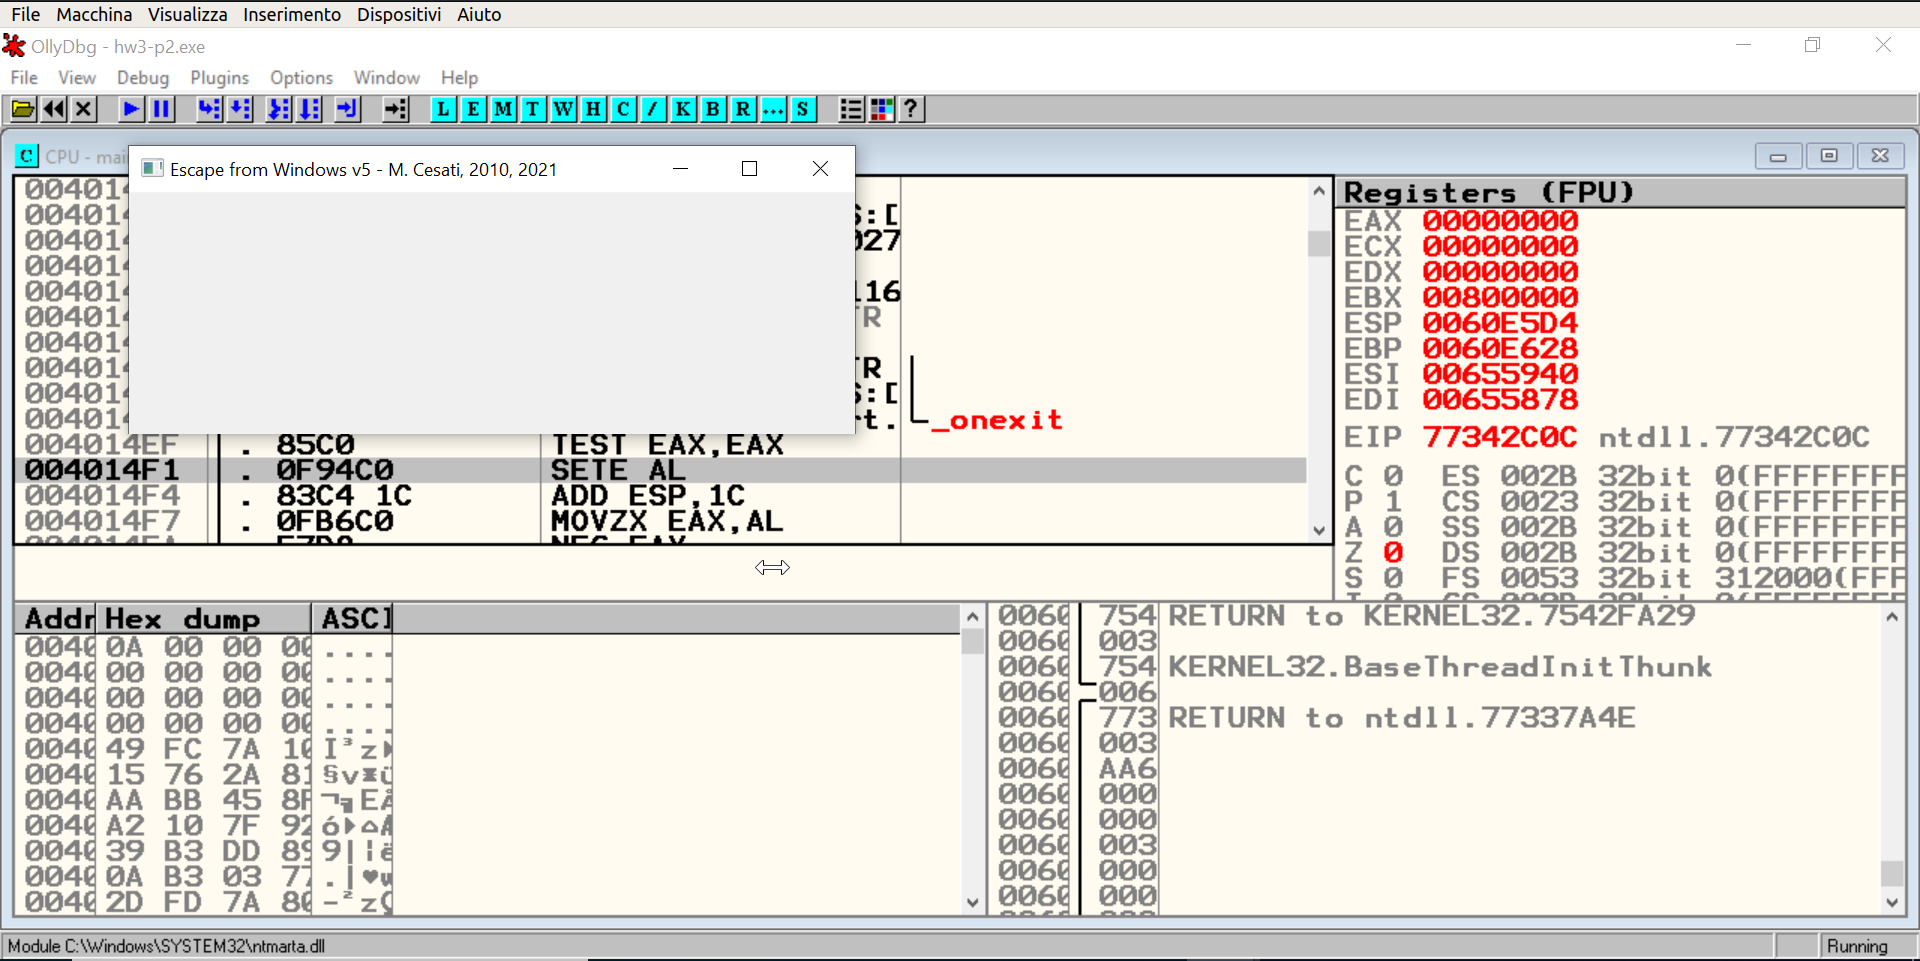
\includegraphics[width=\textwidth]{before_crash}\\
\textit{Immagine catturata pochi istanti prima del crash di OllyDB.}
\end{figure}
Si torna quindi su \ghidra{} alla ricerca di riferimenti all'\api{} \code{OutputDebugString} nella lista degli \textit{imports}, ma non vengono trovati. Si nota però la presenza delle \api{} \code{LoadLibrary} e \code{GetProcAddress}, anche se sembrano non essere invocate nel codice. \\
Si deve capire dove potrebbe avvenire l'invocazione di \code{OutputDebugString}: la finestra viene mostrata ma è incompleta e perciò si procede controllando i blocchi di \code{WM_CREATE}, \code{WM_SIZE} e \code{WM_PAINT} della \key{window\_procedure}. Seguendo questa strada, vengono messi 3 \textit{breakpoints} su \ollydb{} ai seguenti indirizzi:
\begin{enumerate}
\item \key{0x401eb0}: prima istruzione del blocco \code{WM_CREATE}
\item \key{0x401fa8}: prima istruzione del blocco \code{WM_SIZE}
\item \key{0x402108}: prima istruzione del blocco \code{WM_PAINT}
\end{enumerate}
Premendo \key{F9}, si raggiunge il primo \textit{breakpoint}. Premendo di nuovo \key{F9}, si raggiunge il secondo e la finestra viene mostrata: si deduce che l'invocazione non è all'interno del blocco \code{WM_CREATE}. Premendo di nuovo \key{F9}, il terzo \textit{breakpoint} non viene raggiunto e l'esecuzione termina: si controlla quindi il blocco \code{WM_SIZE}, procedendo in parallelo con \ghidra{} e \ollydb{}.\\
Al termine di questo blocco c'è una funzione che \ollydb{} riesce a raggiungere: \code{FUN_00404000_invoke_outputDebugString}. Qui si accede all'area di memoria all'indirizzo \key{0x405020} e si decodificano i byte presenti. La decodifica avviene con le seguenti istruzioni:
\begin{myverb}
XOR EDX, EDX
label:
MOV EAX, dword ptr [EDX*0x4 + 00405020]
XOR EAX, 0x89a3fa2b
ROR EAX, 0x9
MOV dword ptr [EDX*0x4 + 00405020], EAX
ADD EDX, 0x1
CMP EDX, 0xe
JNZ label
\end{myverb}
Dopo aver decodificato quel blocco di codice, si passa ad eseguirlo con una \code{JMP}. Il codice decodificato è il seguente:
\begin{figure}[H]
\centering 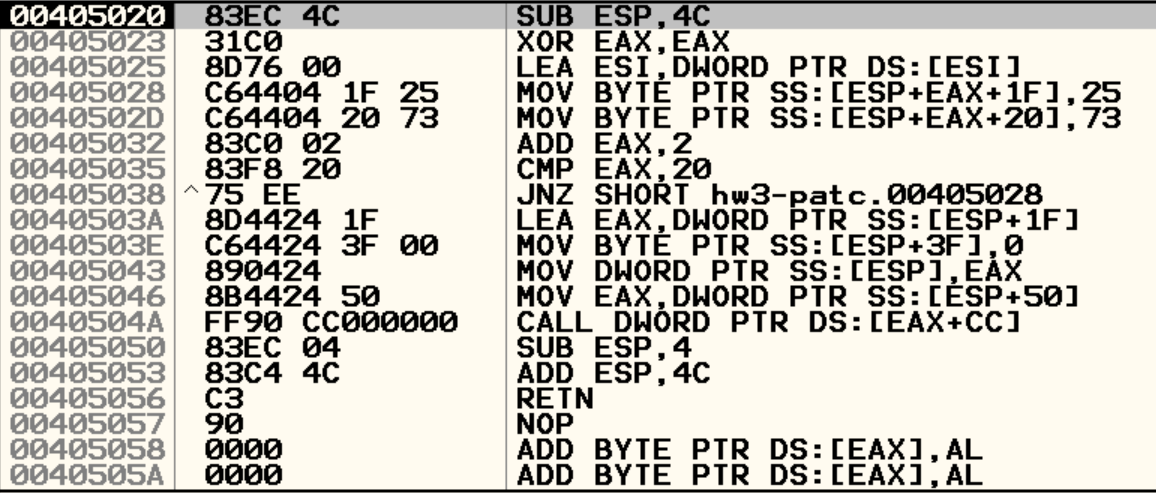
\includegraphics[width=\textwidth]{istructions_at_00405020}
\end{figure}
Questo set di istruzioni genera sullo stack una stringa composta da 16 \code{"\%s"} e invoca la funzione contenuta all'indirizzo \key{0x407020 + 0xcc}, che sarà sicuramente \code{OutputDebugString}. Su \ghidra{} ci sono molte referenze all'indirizzo \key{0x407020}, tra cui alcune scritture nella funzione \code{FUN_00401830_init_appds}: è l'indirizzo della struttura dati che gestisce l'applicazione, già vista nell'\textit{homework2}. Questa struttura dati viene qui estesa e, in particolare, all'offset 204 verrà memorizzato l'indirizzo di \code{OutputDebugString}, in base a quanto detto precedentemente:
\begin{figure}[H]
\centering 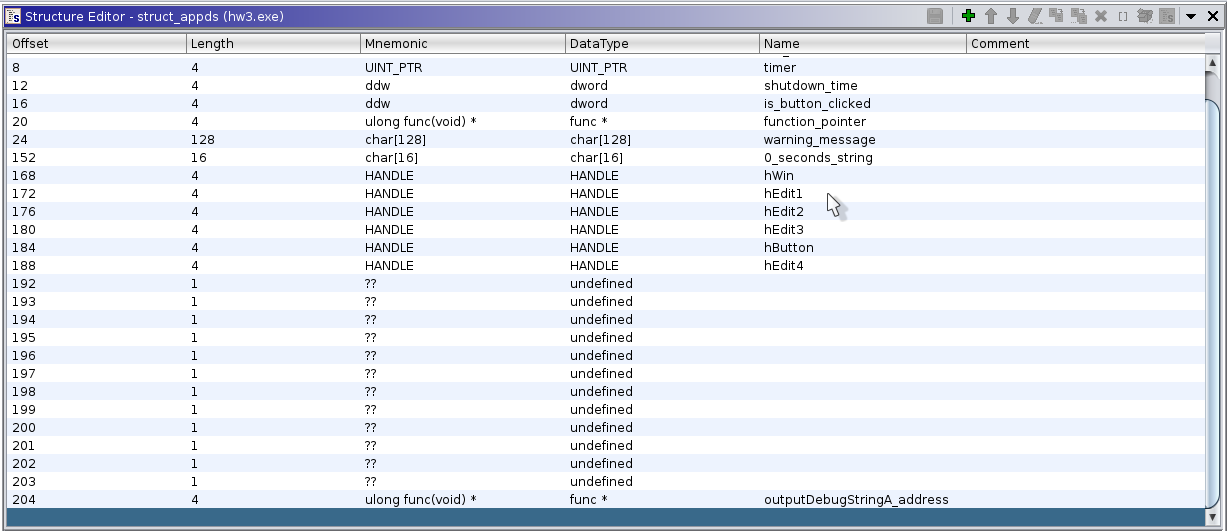
\includegraphics[width=\textwidth]{struct_appds}
\end{figure}
Questo nuovo campo della struttura dati viene inizializzato proprio nella funzione \code{FUN_00401830_init_appds}, impostandolo al valore di ritorno di \code{FUN_004016f0_retrieve_OutputDebugStringAddress}. Sono presenti meccanismi di anti-disassemblaggio ma, alla fine, viene caricata la libreria \code{kernel32.dll} per recuperare l'indirizzo di \code{OutputDebugString}; questo indirizzo viene infine restituito. Le stringhe usate vengono costruite sullo stack un carattere alla volta in modo da nosconderle all'analisi statica di base.\\ 
Continuiamo quindi l'analisi applicando una terza \textit{patch} all'eseguibile, sostituendo l'invocazione della funzione \code{FUN_00404000_invoke_outputDebugString} all'interno del blocco di gestione di \code{WM_SIZE} della \key{window\_procedure} con una istruzione di \code{NOP}.\\
Con questa \textit{patch}, \ollydb{} non crasha, ma i meccanismi di anti-debugging non sono finiti: viene infatti mostrata una finestra di errore.
\begin{figure}[H]
\centering 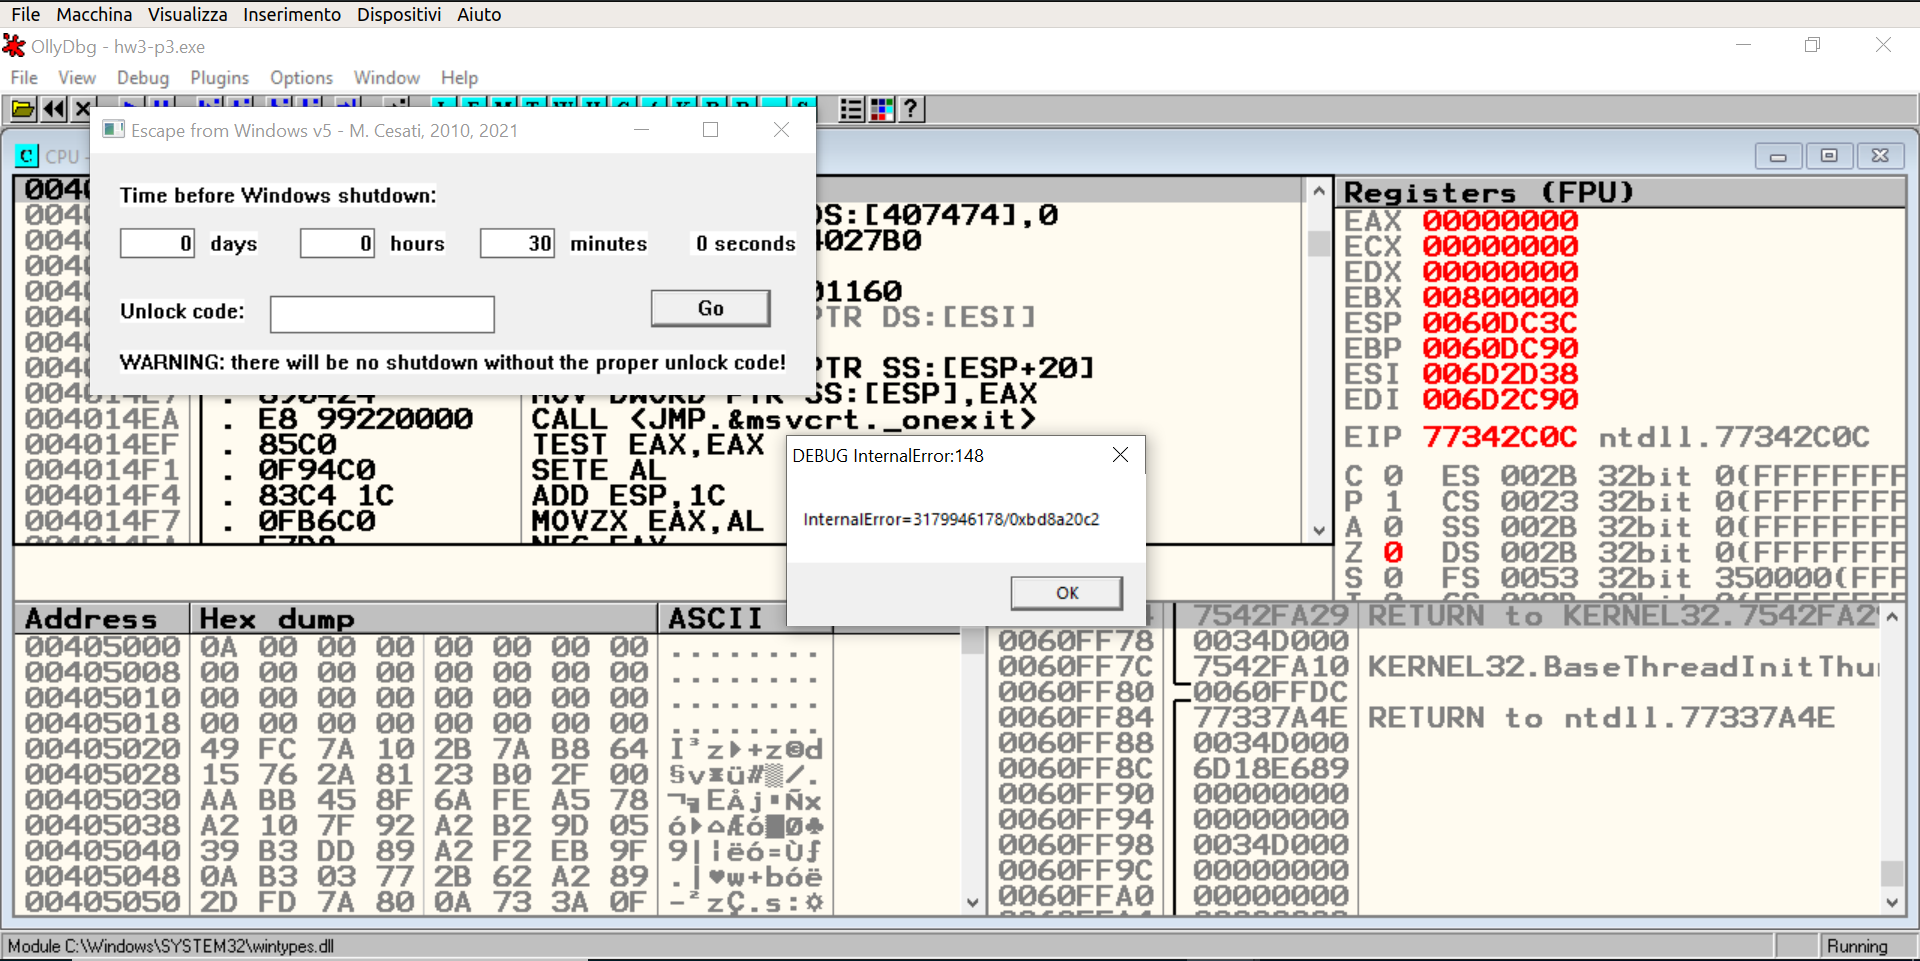
\includegraphics[width=\textwidth]{debug_patch_error}
\end{figure}
A questo punto rimangono solo due funzioni sospette che non sono ancora state analizzate:
\begin{itemize}
\item \code{FUN_00401560_create_and_load_file_mapping} invocata nel \code{FUN_004024e0_win_main}. Qui viene aperto l'eseguibile con \code{CreateFileA} per poi creare un suo \textit{file mapping object} con \code{CreateFileMapping}. Il valore di ritorno di quest'ultima invocazione è passato alla funzione \code{MapViewOfFile} per caricare il \textit{file mapping object} nell'\textit{address space} del processo. Il valore restituito è l'indirizzo in cui viene caricato e viene memorizzato all'\textit{offset} 196 della struttura dati \code{struct_appds}; quel campo viene rinonimato \key{starting\_file\_view\_address}. In questa funzione, viene inizializzato anche un altro campo della struttura: il campo all'\textit{offset} 200 viene impostato pari al valore del campo \code{nFileSizeLow} della struttura dati \code{BY_HANDLE_FILE_INFORMATION} passata all'invocazione \code{GetFileInformationByHandle}. Questo campo, nel nostro caso, è in grado di memorizzare l'intera taglia dell'eseguibile. Il campo della struttura dati viene rinonimato in \key{nFileSizeLow}.

\item la funzione \code{FUN_004016b0_compute_checksum} invocata nel blocco \code{WM_CREATE} in \code{FUN_00401de0_window_procedure}. In questa funzione si parte dall'indirizzo memorizzato nel campo \key{starting\_file\_view\_address} e ci si sposta di 1024 bytes: si ricade all'inizio della sezione \key{.text}. Si memorizza in \code{EAX} il valore del campo \key{nFileSizeLow} della struttura dati \key{struct\_appds}, lo si divide per 4 e si sottrae \key{0x100}: si sta contando il numero di \key{dword} presenti del file, escludendo quelle contenute nei primi 1024 bytes. Poi parte un ciclo in cui si calcola lo \key{XOR} di tutte queste \key{dword}: si sta praticamente calcolando un \textbf{checksum}. Il valore finale viene salvato all'offset 192 della struttura dati; quel campo viene quindi chiamato \key{checksum}.
\begin{figure}[H]
\centering 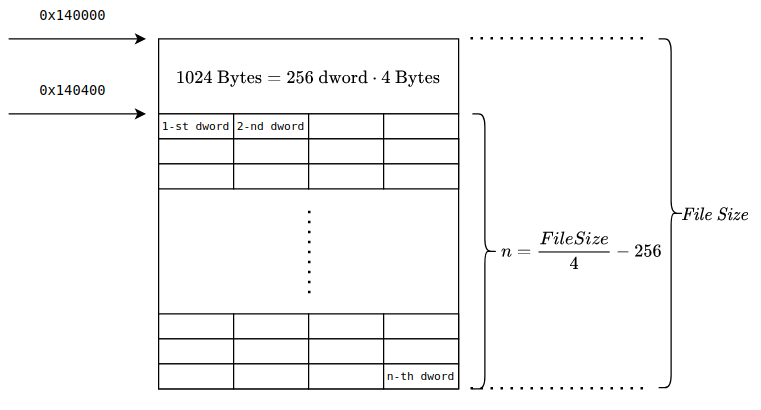
\includegraphics[width=0.7\textwidth]{checksum_computation}\\
\textit{Solo le $n$ parole rappresentate vengono incluse nel calcolo del checksum.}
\end{figure}
\end{itemize} 

\begin{figure}[H]
\centering 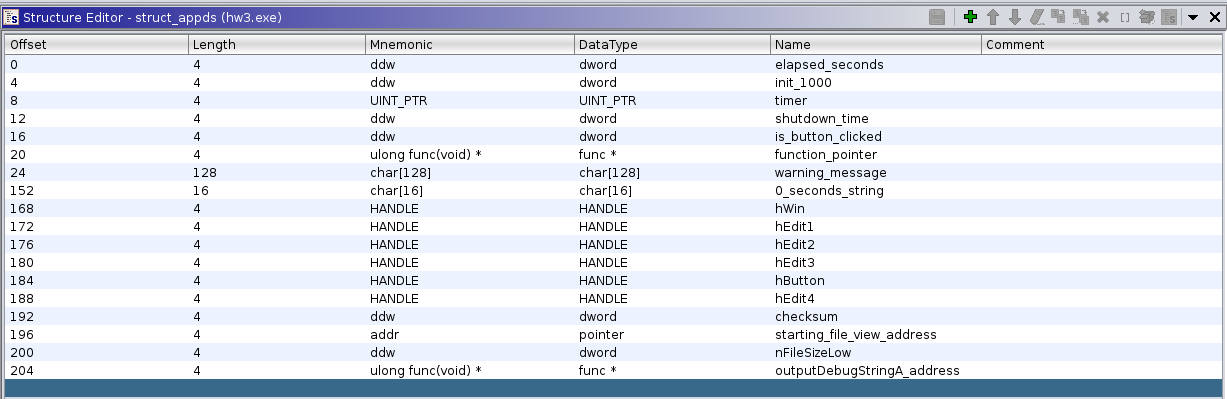
\includegraphics[width=\textwidth]{complete_struct_appds}\\
\textit{Struttura dati completa}
\end{figure}

Avendo \textit{patch-ato} il file, il \key{checksum} calcolato sarà sicuramente diverso da quello atteso, ovunque questo venga controllato. Per questo motivo, si recupera il file originale per cercare di ottenere il valore valido e applicare in seguito una nuova \textit{patch}. Nonostante i \textit{breakpoints} software modifichino il codice sostituendo il codice operativo dell'istruzione in cui fermarsi con quello di \code{INT3}, si possono comunque usare in questo caso: infatti la modifica avviene al codice caricato in memoria, mentre il \key{checksum} è calcolato sul \textit{file mapping object} ottenuto leggendo il file sul disco. Sono inoltre necessari soltanto 2 \textit{breakpoints}:
\begin{itemize}
\item in \code{FUN_00401dc0_check_debugger_FS[30]}, all'indirizzo \key{0x401dce}. Dopo le istruzioni:
\begin{myverb}
MOV EDX, dword ptr FS:[0x30]
MOV EDX, dword ptr [EDX + 0x2]
\end{myverb}
in \code{EDX} ci sarà il valore \code{FFFF0001} e dovrà essere cambiato in \code{FFFF0000}.

\item in \code{FUN_004016b0_compute_checksum}, all'indirizzo \key{0x4016e2}: qui si potrà leggere in \code{ECX} il \key{checksum} valido.
\end{itemize}
Il valore letto è \code{74ee8f1f}. Si procede ricaricando l'eseguibile con le 3 \textit{patches} fatte per poi aggiungerne una quarta: si sostituiscono le prime istruzioni di \code{FUN_004016b0_compute_checksum} con:
\begin{myverb}
MOV dword ptr [4070e0], 74eebf1f
RETN
\end{myverb}
%
%A questo punto, però, vediamo che le \textit{edit text} e il \textit{bottone} sono stati creati correttamente: questo significa che il blocco di gestione \code{WM_CREATE} viene eseguito almeno fino alla creazione di questi elementi. Mettendo un breakpoint all'indirizzo \key{0040248c}, vediamo che la funzione che fa comparire il messaggio di errore è \code{FUN_00401b30_set_timer}. Qui, però, viene solo inizializzato il timer, quindi l'errore deve essere all'interno della funzione che \code{SetTimer} riceve come quarto parametro per specificare il comportamento del timer ogni volta che passa il tempo specificato come terzo parametro. Si tratta della funzione \code{FUN_004019a0_tick_update_timer}. Questa funzione, prima di terminare, controlla il valore del campo \code{elapsed_seconds} della nostra struttura dati \code{struct_appds} e viene messo in \code{AND} con il valore 7 e se il risultato è 0 viene invocata una nuova funzione prima di terminare. Il valore nella struttura dati è inizialmente 0, quindi il risultato sarà sempre 0: seguiamo quindi la funzione \code{FUN_004042a0_show_patched_error}. L'analisi di questa funzione non è stata approfondita, ma qui viene effettivamente invocata la \code{MessageBoxA} con stringhe che hanno il formato di quelle mostrate dall'applicazione. Potrebbe valere la pena provare a patchare l'invocazione della funzione per vedere se il problema viene effettivamente risolto. Viene quindi sostituita la \code{CALL} all'indirizzo \textit{00401a21} con una istruzione \code{NOP}. \\
Questa \textit{patch}, insieme a tutte le altre, sblocca l'esecuzione dell'applicazione con \ollydb{}.\\

Si procede quindi mettendo un \textit{breakpoint} sulla prima istruzione della funzione che viene invocata al termine del timer, memorizzata nel campo \key{function\_pointer} della struttura \key{struct\_appds}. Questo campo viene inizializzato nella funzione \code{FUN_00401830_init_appds} con l'indirizzo della funzione \code{FUN_004040e0_timer_proc_end}. Anche qui sono presenti molti meccanismi anti-disassemblaggio, quindi è conveniente procedere in parallelo con \ollydb{} e \ghidra{}. All'indirizzo \key{0x4041f7} c'è l'invocazione dell'\api{} \code{GetDlgItemTextA}, utilizzata per recuperare il codice inserito dall'utente. Il buffer specificato è il registro \code{ESI}, mentre il numero di bytes letti verrà inserito in \code{EAX}. L'esecuzione continua poi effettuando la stessa operazione di decodifica vista nel caso di \code{FUN_00404000_invoke_outputDebugString}, accedendo però all'area di memoria in \key{0x4050c0}:
\begin{myverb}
XOR ECX, ECX
label:
MOV EDX, dword ptr [ECX*0x4 + 004050c0]
XOR EDX, 0x89a3fa2b
ROR EDX, 0x9
MOV dword ptr [ECX*0x4 + 004050c0], EDX
ADD ECX, 0x1
CMP ECX, 0x34
JNZ label
\end{myverb}
A questo punto, bisogna proseguire usando soltanto \ollydb{}: le istruzioni su \ghidra{} sono codificate. Dopo l'operazione di decodifica, l'esecuzione continua con una \code{CALL} a quell'indirizzo. Qui vengono fatti dei controlli in modo sequenziale: prima si controlla se la lunghezza della stringa inserita dall'utente sia uguale a 9, poi ne vengono controllati i caratteri uno alla volta, terminando al primo esito errato. Tuttavia, questi 9 controlli non sono fatti \textit{in chiaro}: ogni carattere del codice dell'utente viene messo in \code{XOR} con uno specifico byte e si controlla che il risultato dell'operazione sia uguale a un certo risultato atteso. In particolare, la lista dei byte con cui il codice dell'utente è messo in \code{XOR} è:
\begin{myverb}
{ 0x3f, 0x28, 0x2f, 0xa5, 0x5d 0x47, 0x3d, 0x4f, 0x3f }
\end{myverb}
Chiamiamo questi byte $k_i$ $\forall i \in [0..8]$.\\
La lista degli output attesi, invece, è:
\begin{myverb}
{ 0x0c, 0x5a, 0x61, 0xc0, 0x2e 0x13, 0x0d, 0x70, 0x1e }
\end{myverb}
Chiamiamo questi byte $y_i$ $\forall i \in [0..8]$.\\
Chiamiamo inoltre i caratteri della password attesa $x_i$ $\forall i \in [0..8]$.\\

Le precedenti informazioni bastano a ricostruire la password attesa: per le proprietà dello \code{XOR}, infatti, si ha che: 
\[
y_i = x_i \xor k_i \implies y_i \xor k_i = x_i \xor k_i \xor k_i = x_i \xor 0 = x_i \implies y_i \xor k_i = x_i 
\]

\begin{minipage}{0.45\textwidth}
\begin{figure}[H]
\centering 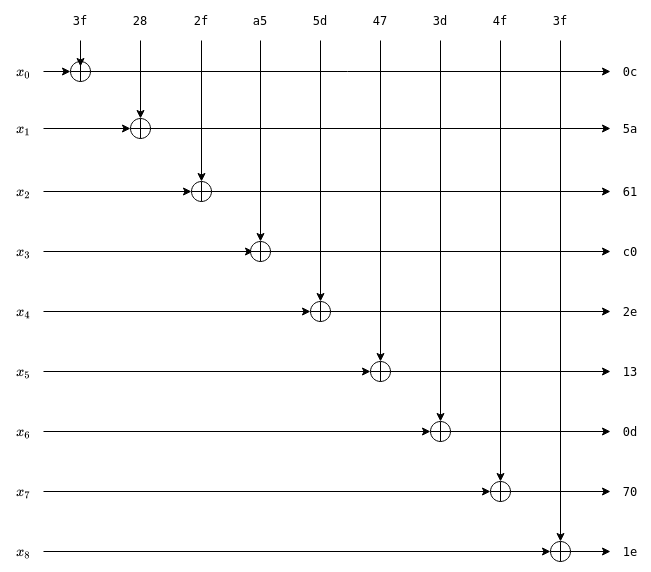
\includegraphics[width=\textwidth]{expected_xor_schema}
%\caption{\textit{Schema con cui funziona l'applicazione.}}
\end{figure}
\end{minipage}\hfill	
\begin{minipage}{0.45\textwidth}
\begin{figure}[H]
\centering 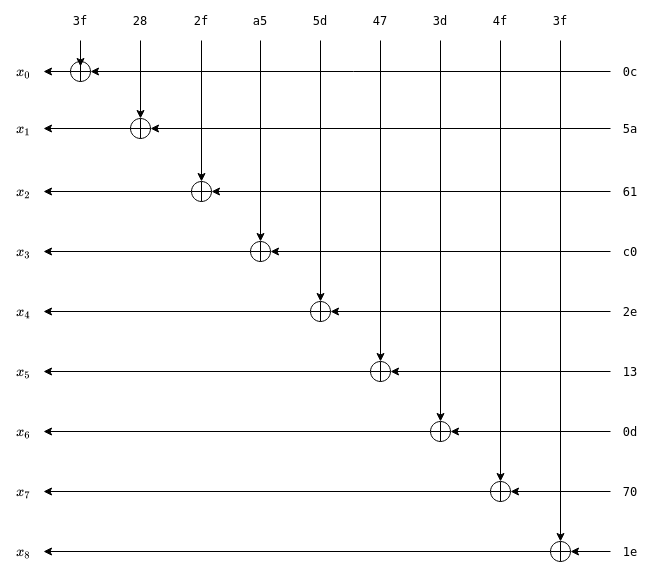
\includegraphics[width=\textwidth]{xor_property}
%\caption{\textit{Invertendo la direzione, si può risalire alla password che sblocca l'applicazione.}}
\end{figure}
\end{minipage}\bigskip

\begin{minipage}{0.45\textwidth}
\textit{Schema con cui funziona l'applicazione.}
\end{minipage}\hfill
\begin{minipage}{0.45\textwidth}
\textit{Invertendo la direzione, si può risalire alla password che sblocca l'applicazione.}
\end{minipage}

\newpage
\section{Verifica}
Per verificare che le informazioni raccolte siano giuste, è stato creato un semplice script \textit{python} per ricostruire la password:
\begin{myverb}
def decrypt_byte(hex1, hex2):
    tmp = int(hex1, 16) ^ int(hex2,16)
    return chr(tmp)

if __name__ == '__main__':
    hex_key = ['3f', '28', '2f', 'a5', '5d', '47', 
            '3d', '4f', '3f']
            
    expected_outputs = ['0c', '5a', '61', 'c0', '2e',
            '13', '0d', '70', '1e']
    s = ''
    for k_i,y_i in zip(hex_key, expected_outputs):
        s += decrypt_byte(k_i, y_i)
    print('The password is:', s)
\end{myverb}
La password che viene stampata dallo script è \textbf{3rNesT0?!}. Inserendola nell'apposita \textit{edit text}, la macchina virtuale \textit{Windows} viene effettivamente arrestata al termine del \textit{countdown}.

\end{document}